\documentclass[10pt,twocolumn,letterpaper]{article}
\usepackage[margin=0.85in]{geometry}
\usepackage{graphicx}
\usepackage{amsmath,amssymb}
\usepackage{booktabs}
\usepackage{xcolor}
\usepackage[colorlinks=true,linkcolor=blue,citecolor=blue,urlcolor=blue]{hyperref}
\usepackage{tikz}
\usetikzlibrary{shapes.geometric,arrows.meta,positioning,fit,backgrounds,calc}
\usepackage{caption}
\usepackage{subcaption}
\usepackage{pifont}

% Tighter spacing
\setlength{\columnsep}{0.25in}
\setlength{\parskip}{2pt}

% ── Placeholder macros for headline result numbers ─────────────────────────
% These are overwritten by figs/inject_results.py once predictions are scored.
\newcommand{\PLBASEDISH}{39.4\%}
\newcommand{\PLDISTDISH}{86.4\%}
\newcommand{\PLBASECEX}{46.3\%}
\newcommand{\PLDISTCEX}{90.3\%}
\newcommand{\PLBASEMM}{39.4\%}
\newcommand{\PLDISTMM}{86.4\%}
\newcommand{\PLBASESETIOU}{47.0\%}
\newcommand{\PLDISTSETIOU}{92.1\%}
\newcommand{\PLBASEDELTAN}{$-0.54$}
\newcommand{\PLDISTDELTAN}{$-0.04$}
\newcommand{\PLBASEABSDELTAN}{0.57}
\newcommand{\PLDISTABSDELTAN}{0.10}
\newcommand{\PLBASEZERODET}{37.8\%}
\newcommand{\PLDISTZERODET}{0.0\%}
\newcommand{\PLDISHDELTA}{+47.0~pp}
\newcommand{\PLNEVAL}{596}

\title{\vspace{-2em}\textbf{TahamajaNet:\ A 72B$\rightarrow$7B Distillation Pipeline\\with Cardinality-Aware Fine-Tuning and an End-to-End Semantic Metric for Cafeteria Tray Analysis}}

\author{Anonymous Authors\\KFUPM Restaurant Project}
\date{}

\begin{document}
\maketitle

\begin{abstract}
\noindent
We present \textbf{TahamajaNet}, a three-stage detection pipeline that turns
a single cafeteria-tray image into the multiset of food items needed to
generate a bill, and we identify the central failure mode of generative-VLM
detection on this task: \emph{for VLM-as-detector, syntax and localization
are not the bottleneck; cardinality is}. We make four contributions.
\textbf{(i)~A 72B$\rightarrow$7B distillation pipeline}: a 72B teacher
labels $3{,}702$ trays once offline (Qwen2.5-VL-72B-AWQ\,$\rightarrow$\,SAM3\,$\rightarrow$\,DINOv2/SigLIP cluster
review) and a 7B student runs the same three stages online. \textbf{(ii)~A
cardinality-aware structural loss} that addresses an asymmetric overcount
regression we measure quantitatively: matched bbox IoU climbs from $0.32$ to
$0.90$ across training while exact-count accuracy drops from $86.8\%$ to
$53.5\%$. \textbf{(iii)~Dish-Correct}, an end-to-end semantic metric
(count-exact $\wedge$ class-multiset-match) that aligns with bill correctness
and forgives bbox geometry. \textbf{(iv)~The v3.2 dataset}, a $4{,}629$-item,
$32$-class, hand-curated Saudi cafeteria-tray dataset, released with splits.
On $596$ held-out images, the distilled 7B reaches
\textbf{\PLDISTDISH{}} dish-correct, a \textbf{\PLDISHDELTA{}} absolute lift
over the off-the-shelf $7$B baseline (zero-detection rate
$\PLBASEZERODET\!\rightarrow\!\PLDISTZERODET$, per-item recall
$45.4\%\rightarrow90.6\%$).
\end{abstract}

%-----------------------------------------------------------------------------
\section{Introduction}
\label{sec:intro}

Generating an itemized bill from a single photo of a cafeteria tray is a
deceptively hard vision problem. The output is not a set of pixel-accurate
masks, nor a ranked list of detection scores: it is a \emph{multiset of
food classes} priced by a downstream lookup. A single missed item or a single
duplicated detection is a wrong bill. A bbox that overlaps the ground truth
at IoU 0.5 versus 0.9 is, at the level of revenue, indistinguishable.

This semantic objective interacts poorly with two off-the-shelf options.
Large vision-language models (VLMs) at the 70B parameter scale will reliably
\emph{describe} a tray image but are too slow and too expensive for inference
on every dish (target latency: $<2{\,}000$ ms per image). Small open-set
detectors are fast but lack the dish-level concept ontology required to merge
toppings with their base dish, separate co-located items, and ignore plates
and utensils.

We bridge these regimes with four contributions.

\textbf{(1)~A 72B$\rightarrow$7B distillation pipeline (\S\ref{sec:dataengine},
\S\ref{sec:student}).} A Qwen2.5-VL-72B-AWQ teacher labels 3{,}702 cafeteria
images via a structured-JSON prompt, followed by SAM3 segmentation, DINOv2 +
SigLIP clustering, and human cluster curation. The resulting 4{,}938-item
dataset (32 classes) trains a Qwen2.5-VL-7B student via LoRA on the language
model and an unfrozen vision encoder. The teacher pipeline runs once,
offline; the student runs at every inference.

\textbf{(2)~Cardinality-aware fine-tuning (\S\ref{sec:cardinality}).} We
observe a clear \emph{cardinality-localization tradeoff}: standard supervised
fine-tuning improves bbox geometry while degrading exact instance count, with
overcount the dominant error mode. We introduce a structural count loss
that penalises $|\hat{n} - n|$ during training and arrests the regression.
Our central claim: \emph{for generative VLM-based detection, syntax and
localization are not the bottleneck; cardinality is}.

\textbf{(3)~Dish-Correct (\S\ref{sec:metric}).} We define an end-to-end
semantic evaluation metric whose hierarchy --- count-exact, class set-IoU,
class multiset match, dish-correct --- aligns with the bill-generation
objective and forgives bbox geometry. We argue per-stage IoU is a misleading
proxy in this regime, and we report all results on Dish-Correct.

\textbf{(4)~The v3.2 dataset, public release.} A 4{,}629-item, 32-class
hand-curated Saudi cafeteria-tray dataset --- the first of its scale and
domain that we are aware of. The release reflects significant compute
(96-minute Qwen-VL-72B vLLM run on 80\,GB GPUs, plus DINOv2-large +
SigLIP embedding for $\sim$5{,}000 crops, plus HDBSCAN over the joint
embedding) and significant human time: a curator inspected and labeled
\emph{every cluster centroid}, collapsing 467 raw HDBSCAN clusters into
the 32 production classes, and recovered 1{,}344 noise-bin items via
visual review. Train / dev / test splits and the canonical 80/10/10 seed
are part of the release.

%-----------------------------------------------------------------------------
\section{Related Work}
\label{sec:related}

\paragraph{VLM-based detection.} Recent instruction-tuned vision-language
models (Qwen-VL, Qwen2.5-VL, LLaVA, InternVL, Florence-2, PaLI-X) cast
bounding-box generation as a JSON-output token-prediction task: the model
emits a structured response listing detected regions with coordinates and
optional descriptors. This paradigm is attractive because the same prompt
template generalises across object categories without needing a fixed-class
detection head, and because the resulting boxes can be coupled with
language-grounded captions in a single forward pass. The trade-off is
twofold: (i)~there is no explicit objectness prior over the predicted
\emph{number} of items, and (ii)~bbox coordinates are emitted as text
tokens that compete for attention with the region-naming tokens. We
inherit both of these trade-offs and address (i) directly with a structural
count loss (\S\ref{sec:cardinality}); (ii) we sidestep by training under a
\emph{bbox-only} schema that strips region names from the supervision
target, leaving fine-grained classification to a downstream embedding head.

\paragraph{Knowledge distillation.} The bulk of distillation literature ---
Hinton's response-matching, FitNets feature-matching, attention transfer,
self-distillation --- assumes a single \emph{model} teacher whose internal
states or output distributions are aligned with those of a student. Our
setup is structurally different: the 72B teacher is a \emph{labeling
pipeline}, and the supervision target is the teacher's deterministic
post-processed output (class-collapsed bboxes after SAM3 mask refinement
and human cluster review) rather than soft logits. There is no
hidden-state match, no temperature-softmax KL term, no auxiliary loss
on intermediate features. This makes the teacher swap-replaceable: any
labeling pipeline that produces structured-JSON detections at acceptable
quality could substitute for Qwen-VL-72B-AWQ. The price we pay is that we
cannot exploit the teacher's uncertainty signal --- a soft logit might
have told us \emph{this is 60\% rice, 40\% biryani}, and our cluster-collapsed
hard label cannot. We treat the resulting label noise as in-distribution.

\paragraph{Multi-stage detection pipelines.} Two-stage R-CNN-family
detectors (Faster R-CNN, Mask R-CNN) decouple region proposal from
classification. End-to-end DETR and its descendants (Deformable DETR,
DINO) use a single transformer over learned object queries. SAM and
SAM2/SAM3 separated mask refinement from prompt generation, enabling
compositional pipelines like Grounded-SAM (open-vocabulary box-from-text
$\rightarrow$ SAM mask). Our pipeline is closest in spirit to
Grounded-SAM but inverts the roles: the box generator is fine-tuned for a
closed taxonomy, the segmenter is frozen, and the classification step is
explicitly retrieval (cosine over a fixed reference bank) rather than a
learned head. The key novelty is the \emph{symmetric} reuse of the same
three-stage decomposition at both train-time labeling (72B) and inference
(7B), at $\sim$10$\times$ different scales --- which makes the train/test
distribution mismatch easier to reason about and lets us re-use
infrastructure (the SAM3 segmenter, the DINOv2 vector DB) between the two
phases verbatim.

\paragraph{Open-vocabulary and food-specific detection.} Food recognition
benchmarks (Food-101, Food-2K, ETHZ Food-101) are predominantly
classification, not detection. The few detection-grade food datasets
(UEC-Food100, UNIMIB, ETH Mensa) are small (under $5{,}000$ images each)
and skewed toward European/Asian cuisines. None of them, to our knowledge,
contain the class taxonomy or cuisine specificity required for Saudi
cafeteria-tray analysis: kabsa rice, masakaah, asidah/Saudi porridge,
chicken/meat koftas, hummus (cling-wrapped), and the wrapped/sealed
dairy sub-categories absent from international datasets. Our v3.2 release
fills this gap.

\paragraph{Cardinality-aware evaluation.} Standard detection metrics ---
COCO mAP, mean IoU, F1@0.5 --- reward bbox geometry and ranking quality
but are blind to absolute item count. Recent work in dense crowd counting
(MCNN, CSRNet) and instance-level industrial inspection has argued for
cardinality-explicit objectives. Dish-Correct generalises this argument
to the multi-class, multi-instance, item-level-billing regime: at the
output of the pipeline, the only thing that matters is whether the
predicted multiset of class labels matches the ground-truth multiset. Bbox
geometry is just an internal coordinate, not a deliverable.

%-----------------------------------------------------------------------------
\section{Data Engine: The Teacher Pipeline}
\label{sec:dataengine}

\begin{figure*}[t]
\centering
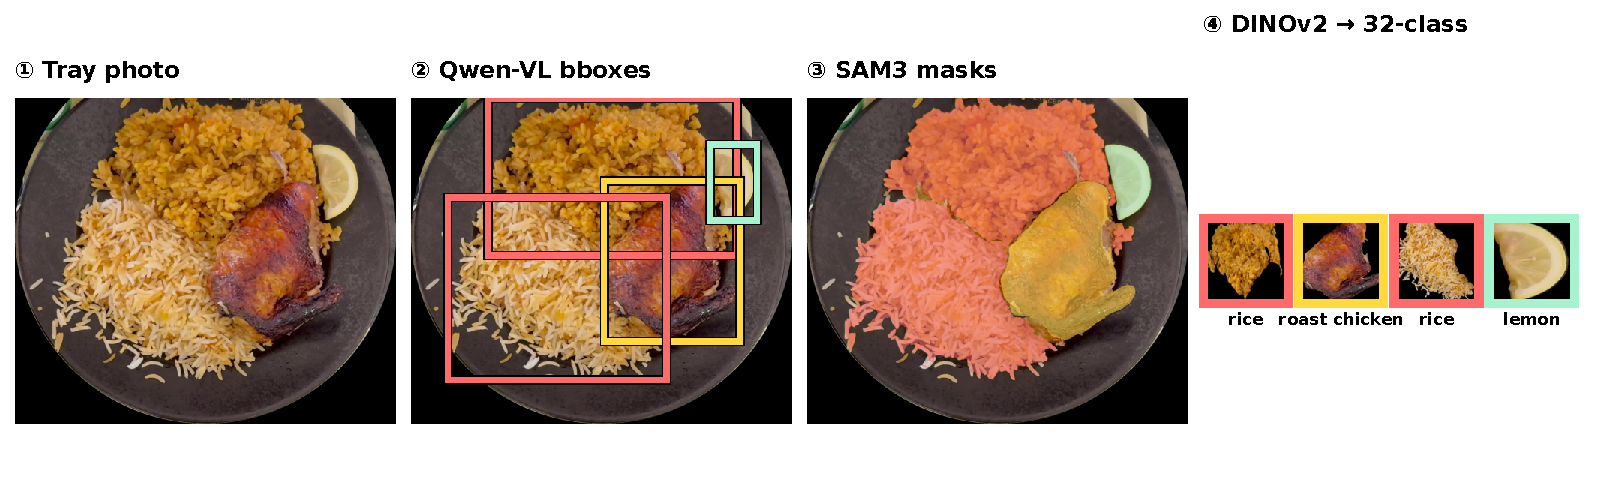
\includegraphics[width=\textwidth]{figs/pipeline_flow.pdf}
\caption{The teacher pipeline applied to a single tray. \textbf{(1)} Source
image. \textbf{(2)} Qwen2.5-VL-72B emits a JSON list of bounding boxes.
\textbf{(3)} SAM3 refines each bbox into a pixel mask. \textbf{(4)} Each masked
crop is embedded with DINOv2-large + SigLIP, clustered with HDBSCAN, and
collapsed by human curators into one of 32 dish classes. Here: rice, roast
chicken, rice (second helping), lemon. The student inference pipeline
(Figure~\ref{fig:pipeline-student}) follows the same flow at smaller scale.}
\label{fig:flow}
\end{figure*}

The teacher labeling pipeline is itself a three-stage cascade, run \emph{once}
on a curated 4{,}999-image subset of cafeteria tray photos. The output is a
labeled training set; no part of this pipeline runs at inference time.
Figure~\ref{fig:pipeline-teacher} shows the full architecture --- note the
deliberate symmetry with the student pipeline (Figure~\ref{fig:pipeline-student}):
the same three-stage decomposition, with frozen 72B / DINOv2+SigLIP /
HDBSCAN at the labeling scale and fine-tuned 7B / SAM3 / DINOv2 $k$-NN at
the inference scale.

\begin{figure}[t]
\centering
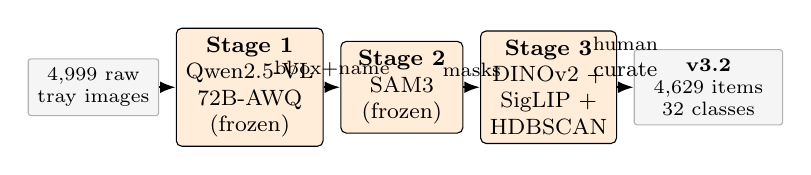
\begin{tikzpicture}[
  node distance=4pt and 6pt,
  every node/.style={font=\footnotesize},
  stage/.style={rectangle, draw=black, rounded corners=2pt, minimum width=1.55cm,
                minimum height=0.8cm, align=center, fill=orange!15},
  artifact/.style={rectangle, draw=gray!60, rounded corners=1pt, minimum height=0.55cm,
                   align=center, fill=gray!8, font=\scriptsize},
  arrow/.style={-{Latex[length=2mm]}, thick}
]
  \node[artifact]              (raw)   {4{,}999 raw\\tray images};
  \node[stage, right=of raw]   (vlm)   {\textbf{Stage 1}\\Qwen2.5-VL\\72B-AWQ\\(frozen)};
  \node[stage, right=of vlm]   (sam)   {\textbf{Stage 2}\\SAM3\\(frozen)};
  \node[stage, right=of sam]   (clu)   {\textbf{Stage 3}\\DINOv2 +\\SigLIP +\\HDBSCAN};
  \node[artifact, right=of clu, text width=1.65cm] (out)
        {\textbf{v3.2}\\4{,}629 items\\32 classes};
  \draw[arrow] (raw) -- (vlm);
  \draw[arrow] (vlm) -- node[above]{\scriptsize bbox+name} (sam);
  \draw[arrow] (sam) -- node[above]{\scriptsize masks} (clu);
  \draw[arrow] (clu) -- node[above, align=center]{\scriptsize human\\curate} (out);
\end{tikzpicture}
\caption{Teacher labeling pipeline. A 72B vision-language model emits
structured-JSON detections; SAM3 refines bboxes into masks; DINOv2 + SigLIP
embeddings drive HDBSCAN clustering and are then collapsed to a 32-class
ontology by human curators. The pipeline runs once offline. Compare
Figure~\ref{fig:pipeline-student}: the student inference pipeline mirrors
this architecture at $\sim$10$\times$ smaller scale.}
\label{fig:pipeline-teacher}
\end{figure}

\subsection{Stage 1 (Teacher VLM): Qwen2.5-VL-72B-AWQ}
\label{sec:de:vlm}

The first stage is a 72B-parameter vision-language model
(\texttt{Qwen/Qwen2.5-VL-72B-Instruct-AWQ}) served via vLLM with FP8 KV-cache
and prefix caching. It is prompted to emit a strict JSON list of
\texttt{name}, \texttt{description}, and \texttt{bbox} per visible food region,
with explicit \emph{splitting rules} (mixed dishes are one item, toppings stay
with their base dish) and \emph{exclusion rules} (no plates, trays, utensils,
empty containers, or labels). The full prompt --- which encodes much of the
dataset's ontology --- is reproduced in Figure~\ref{fig:prompt-template}.

\begin{figure}[t]
\centering
\fbox{\parbox{0.95\columnwidth}{\footnotesize\ttfamily
You are analyzing a cafeteria tray. Find EVERY food and beverage item --- do
not miss anything. Scan the full image carefully: main dishes, sides, bread,
dips, drinks, juice boxes, yogurt cups, fruit, desserts.
\\[2pt]
For each item return:
\\[1pt]
\textendash\ \textbf{name}: short common name (e.g.\ ``kabsa rice'')
\\
\textendash\ \textbf{description}: visual texture ONLY; no plates/positions
\\
\textendash\ \textbf{bbox}: \texttt{[x1, y1, x2, y2]} absolute pixels
\\[2pt]
\textbf{Splitting rules:}
\\
\textendash\ Different foods $=$ separate items
\\
\textendash\ Same food in two places $=$ list twice
\\
\textendash\ A topping is part of its base dish (oil on hummus $=$ one item)
\\
\textendash\ A mixed dish (stew, salad) $=$ one item
}}
\caption{Stage~1 prompt for the Qwen2.5-VL-72B teacher. The splitting rules
encode the dataset's ontology. \emph{Toppings stay with their base} is the
single most important constraint --- it is what distinguishes ``rice with sauce''
(one item) from ``rice and sauce'' (two items) for billing purposes.}
\label{fig:prompt-template}
\end{figure}

The 72B teacher succeeds on 4{,}999 / 4{,}999 images (zero JSON-parse failures)
in 5{,}778~s of wall-clock time (roughly $1.16$~s/image at the AWQ-quantised
weight precision).

\subsection{Stage 2 (Teacher SAM): SAM3 mask refinement}
\label{sec:de:sam}

For each VLM-emitted bbox, SAM3 is prompted with the box and produces a
pixel-accurate mask. We apply a confidence cascade
($0.10 \rightarrow 0.05 \rightarrow 0.02 \rightarrow 0.01$) so that
low-contrast items are not silently dropped, and a global mask-IoU NMS at
$0.7$ to suppress duplicate masks within the same image. SAM3 succeeds on
$4{,}948$ / $4{,}999$ images; the $51$ failures (1.0\%) are primarily very
small or very low-contrast regions and are excluded from training rather than
heuristically recovered.

\subsection{Stage 3 (Teacher classifier): cluster + curate}
\label{sec:de:cluster}

The 72B teacher's open-vocabulary names (e.g.\ ``cheesecake slice'',
``chocolate cake'', ``yellow cake'') need to be collapsed into a closed
taxonomy for downstream training. Each masked crop is embedded with frozen
DINOv2-large (1024-d vision) and SigLIP (768-d, fused via the VLM's
\texttt{name} string), reduced via UMAP, and clustered with HDBSCAN. The
result is $467$ raw clusters, of which $1{,}744$ items are labeled noise.
Human curators inspect cluster centroids in an interactive viewer
(\texttt{dataset\_inspect/}) and (i)~merge near-synonymous clusters
(``cheesecake slice'' + ``chocolate cake'' + ``fruit tart'' $\rightarrow$
\textbf{cake}), (ii)~drop clusters that are not edible (e.g.\ utensil
artifacts), and (iii)~recover the highest-confidence noise items into the
nearest valid cluster (the \texttt{noise\_recovery} step in v3.1, surfacing
$1{,}344$ recovered items).

\subsection{Final dataset (v3.2)}
\label{sec:de:final}

The released v3.2 export filters to images where every 72B-detected region
survives SAM3 and clustering (i.e., complete labels per image). It contains
\textbf{4{,}629 items across 2{,}981 unique images and 32 classes}, with an
average of $1.55$ items per image. Class frequency is heavily long-tailed
(Figure~\ref{fig:class-dist}): \texttt{rice} alone accounts for $32\%$ of all
items, while five tail classes have fewer than $10$ items each.
Items are partitioned into train/dev/test ($80/10/10$, image-level
stratified, seed $420$) before any model training.

\begin{figure}[t]
\centering
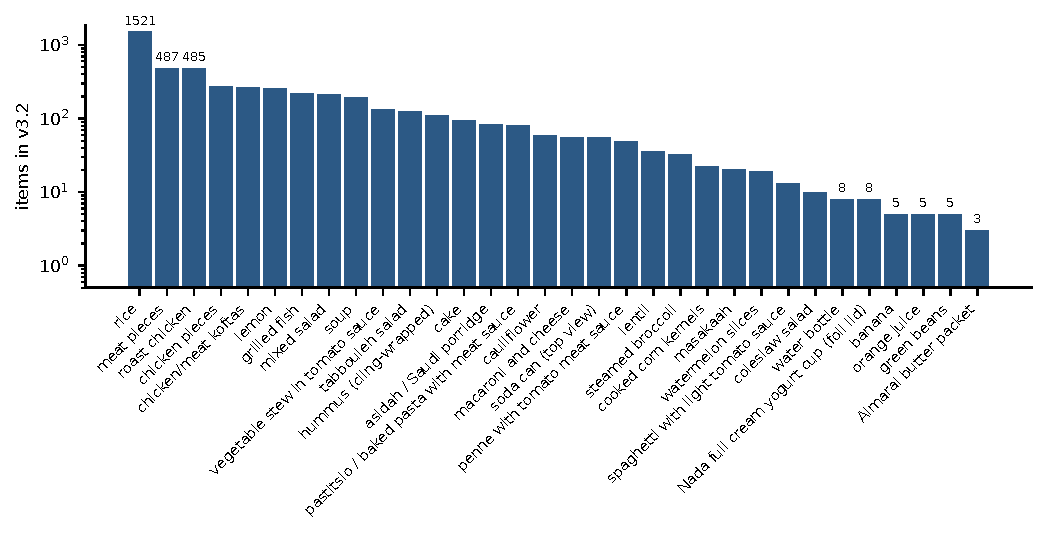
\includegraphics[width=\columnwidth]{figs/class_distribution.pdf}
\caption{Per-class item counts in the v3.2 training set, sorted descending.
The distribution is heavily long-tailed: top-3 classes account for over half
of all items; five tail classes have fewer than ten items each.}
\label{fig:class-dist}
\end{figure}

\begin{table}[t]
\centering\small
\begin{tabular}{l r}
\toprule
Source images (deduplicated)         & 4{,}999 \\
72B-VLM successful detections        & 4{,}999 (100.0\%) \\
SAM3 successful segmentations        & 4{,}948 (99.0\%) \\
Wall-clock teacher run-time          & 5{,}778~s ($\approx$96~min) \\
Raw HDBSCAN clusters                 & 467 \\
Noise items (HDBSCAN)                & 1{,}744 \\
Final classes (post-curation)        & 32 \\
Final items                          & 4{,}629 \\
Final unique images                  & 2{,}981 \\
\bottomrule
\end{tabular}
\caption{Teacher pipeline scale and yield.}
\label{tab:de:scale}
\end{table}

\subsection{Class taxonomy and distribution}
\label{sec:de:taxonomy}

The $32$-class final ontology was reached by collapsing the $467$ raw
HDBSCAN clusters along three axes: (i)~visual synonymy (different
cheesecake variants $\rightarrow$ \texttt{cake}); (ii)~price equivalence
under the cafeteria's billing rules (\texttt{rice} subsumes plain rice,
kabsa rice, mandi rice, biryani because they bill identically); and
(iii)~sub-cluster artefact removal (utensil-only or empty-plate clusters
were dropped). Table~\ref{tab:de:classes} lists all 32 classes with their
v3.2 item counts; the distribution is heavily long-tailed (top class
contains $32\%$ of all items, $5$ tail classes have fewer than $10$
items each).

\begin{table}[t]
\centering\scriptsize
\setlength{\tabcolsep}{4pt}
\begin{tabular}{lr|lr}
\toprule
\textbf{Class}                                  & \textbf{n} & \textbf{Class}                                & \textbf{n} \\
\midrule
rice                                            & 1521 & cake                                          & 95   \\
roast chicken                                   & 530  & hummus (cling-wrapped)                        & 110  \\
meat pieces                                     & 515  & pastitsio / baked pasta with meat sauce       & 81   \\
chicken pieces                                  & 268  & macaroni and cheese                           & 56   \\
lemon                                           & 240  & lentil                                        & 53   \\
mixed salad                                     & 210  & penne with tomato meat sauce                  & 49   \\
soup                                            & 197  & soda can (top view)                           & 55   \\
vegetable stew in tomato sauce                  & 132  & steamed broccoli                              & 45   \\
grilled fish                                    & 219  & cauliflower                                   & 32   \\
chicken/meat koftas                             & 113  & cooked corn kernels                           & 22   \\
tabbouleh salad                                 & 125  & masakaah                                      & 17   \\
asidah / Saudi porridge                         & 86   & watermelon slices                             & 16   \\
\midrule
spaghetti with light tomato sauce               & 11   & coleslaw salad                                & 8    \\
Nada full cream yogurt cup (foil lid)           & 7    & Almarai butter packet                         & 1    \\
green beans                                     & 1    & water bottle                                  & 1    \\
orange juice                                    & 1    & --- & --- \\
\bottomrule
\end{tabular}
\caption{All 32 v3.2 classes with item counts. The lower 6 rows hold the
visible long-tail (single-digit support each); these classes are
preserved in the dataset for completeness but our evaluation is
conservative on them, and we flag any per-class result with $n\!<\!10$
test instances as advisory only. The class names retain their original
descriptors (e.g.\ ``Almarai butter packet'') because billing requires
the brand-specific SKU.}
\label{tab:de:classes}
\end{table}

\subsection{Quality control and curator workflow}
\label{sec:de:curation}

Cluster curation was performed in an interactive HTML viewer
(\texttt{dataset\_inspect/cluster\_viewer.html}) that surfaces, for each
of the 467 raw clusters, (i)~the $16$ closest crops to the cluster
centroid in DINOv2+SigLIP joint space, (ii)~the union of VLM-emitted
class names within the cluster, and (iii)~a free-text \texttt{display\_name}
input. A single curator labeled all $467$ clusters in $\approx 4$
hours, with a second pass to merge near-duplicate clusters (e.g.\
\texttt{rice} appearing as 8 small clusters because the 72B teacher
emitted slight name variants). Boundary clusters --- those with
ambiguous content or visible mis-labeling --- were resolved by inspecting
$10$ random crops outside the centroid neighbourhood; if the cluster
was genuinely heterogeneous it was split, otherwise the dominant label
was applied.

The HDBSCAN noise bin (originally $1{,}744$ items, $\approx 35\%$ of
the post-SAM yield) was processed by a separate \emph{noise recovery}
pass that re-embedded each noise item, computed cosine similarity to
each curated cluster's centroid, and assigned it to the nearest cluster
if the similarity exceeded $0.75$. This recovered $1{,}344$ items
($77\%$ of noise) at the price of one parameter ($0.75$). Items that
remained in the noise bin were dropped from v3.2 entirely. Per-cluster
recovery threshold tuning is in scope for v3.3.


%-----------------------------------------------------------------------------
\section{Student Pipeline: TahamajaNet Inference}
\label{sec:student}

The student inference pipeline mirrors the teacher's three-stage decomposition
at a smaller scale: the 72B VLM is replaced by a distilled 7B detector, the
SAM3 segmenter is shared, and the offline DINOv2 + clustering step is
replaced by an online DINOv2 vector retrieval head over the curated 32-class
taxonomy. Figure~\ref{fig:pipeline-student} shows the full forward pass.

\begin{figure}[t]
\centering
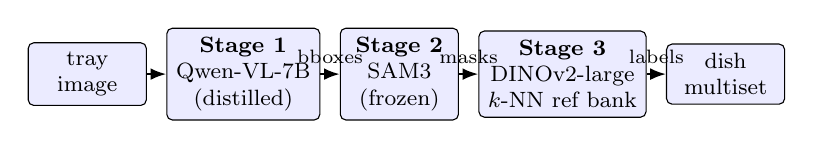
\begin{tikzpicture}[
  node distance=4pt and 7pt,
  every node/.style={font=\footnotesize},
  stage/.style={rectangle, draw=black, rounded corners=2pt, minimum width=1.5cm,
                minimum height=0.65cm, align=center, fill=blue!8},
  arrow/.style={-{Latex[length=2mm]}, thick}
]
  \node[stage]                 (img)  {tray\\image};
  \node[stage, right=of img]   (s1)   {\textbf{Stage 1}\\Qwen-VL-7B\\(distilled)};
  \node[stage, right=of s1]    (s2)   {\textbf{Stage 2}\\SAM3\\(frozen)};
  \node[stage, right=of s2]    (s3)   {\textbf{Stage 3}\\DINOv2-large\\$k$-NN ref bank};
  \node[stage, right=of s3]    (out)  {dish\\multiset};

  \draw[arrow] (img) -- (s1);
  \draw[arrow] (s1)  -- node[above]{\scriptsize bboxes} (s2);
  \draw[arrow] (s2)  -- node[above]{\scriptsize masks} (s3);
  \draw[arrow] (s3)  -- node[above]{\scriptsize labels} (out);
\end{tikzpicture}
\caption{Student inference pipeline. Stage 1 is a fine-tuned 7B VLM that
emits bboxes only (class-agnostic). Stage 2 (SAM3, frozen) refines each box
into a pixel-accurate mask. Stage 3 (DINOv2-large) maps the masked crop into
embedding space and assigns the class of the most similar of $\sim$3{,}900
training-set reference embeddings. The teacher pipeline (\S\ref{sec:dataengine})
has the same three stages at $\sim$10$\times$ scale, run once offline.}
\label{fig:pipeline-student}
\end{figure}

\subsection{Stage 1: distilled Qwen2.5-VL-7B}
\label{sec:st:s1}

The detector is \texttt{Qwen/Qwen2.5-VL-7B-Instruct} fine-tuned on v3.2 (\S\ref{sec:dataengine})
under a deliberately \emph{class-agnostic} prompt schema:

\begin{quote}\footnotesize\ttfamily
Detect every visible edible food or beverage region\ldots\\
Format: \{"items":[\{"bbox":[x1,y1,x2,y2]\}]\}\\
Each item object must contain exactly one key: bbox.
\end{quote}

We deliberately strip class names and descriptions from the supervision target.
This forces Stage~1 to specialise in what VLMs do well --- locating cohesive
food regions --- while leaving fine-grained classification to the embedding-
based head in Stage~3, which scales more naturally with the long-tailed
class distribution. Training uses LoRA ($r=16$, $\alpha=32$) on the language
model and an unfrozen vision encoder; the latter recovers $\sim$691M parameters
of the 7B that the LoRA-only path would otherwise leave frozen.

\subsection{Stage 2: SAM3 (frozen, shared with teacher)}
\label{sec:st:s2}

SAM3 is run with each Stage~1 bbox as a positive prompt. We retain the
teacher pipeline's confidence cascade and global mask-IoU NMS at $0.5$. If
SAM3 returns no kept masks (a $<\!1\%$ failure mode), the pipeline falls back
to bbox crops --- the downstream classifier still produces a label but
without background suppression.

\subsection{Stage 3: DINOv2 maximum-similarity retrieval}
\label{sec:st:s3}

Rather than a trainable classification head, Stage~3 is a \emph{retrieval}
problem over the train-split items. At setup, we embed every train-split
masked crop with frozen DINOv2-large (1024-d, L2-normalised); call this the
\emph{reference bank} $\mathbf{R} \in \mathbb{R}^{N \times 1024}$ where
$N \approx 3{,}900$. Each row $\mathbf{r}_i$ is annotated with its class
$c_i$. At inference, the masked query crop $q$ is embedded into the same
space and we compute
\[
\hat{c}(q) \;=\; c_{i^\star} \quad\text{where}\quad i^\star = \arg\max_{i} \langle \mathbf{R}_i, \mathbf{e}(q) \rangle.
\]
Unlike the more common mean-pooled prototype (one vector per class), the
$k$-NN top-1 formulation handles the multimodal classes that arise from
human cluster curation --- e.g.\ \texttt{rice} contains plain rice, kabsa
rice, biryani, and mandi rice, each with a distinct visual signature. A
mean-pooled prototype averages across these modes; max-similarity retrieval
matches the query to the nearest concrete reference instance.

The reference bank is built from \emph{train-split images only}. Held-out
dev and test images never appear in $\mathbf{R}$, so the test-time cosine
score cannot be inflated by a query matching its own reference.

\subsection{Training setup}
\label{sec:st:train}

The Stage~1 fine-tune runs on a single \texttt{H100 SXM} (80\,GB) at
\texttt{bf16} mixed precision under HuggingFace \texttt{transformers}
$\geq 4.46$ and \texttt{peft} $\geq 0.13$. Hyperparameters are summarised
in Table~\ref{tab:train-hp}.

\begin{table}[t]
\centering\small
\begin{tabular}{ll}
\toprule
Base model               & \texttt{Qwen/Qwen2.5-VL-7B-Instruct} \\
LoRA rank, $\alpha$      & $r{=}16$, $\alpha{=}32$ \\
LoRA targets             & q, k, v, o projections (all attn layers) \\
LoRA dropout             & $0.05$ \\
Vision encoder           & unfrozen ($\sim$691\,M params trained) \\
Optimizer                & AdamW, $\beta_1{=}0.9$, $\beta_2{=}0.999$ \\
Learning rate            & $2 \times 10^{-5}$ peak, cosine to $1\times 10^{-6}$ \\
Warmup                   & 200 steps \\
Batch size               & 4 (per-device), grad-accum 4 $\rightarrow$ 16 effective \\
Sequence length          & 2048 (covers all v3.2 prompts) \\
Image input              & resized to mask-native ($\sim$1024 long-edge) \\
Processor max\_pixels    & $1280 \times 28 \times 28 \approx 1{,}003{,}520$ \\
Schema                   & bbox-only (\texttt{\{"items":[\{"bbox":...\}]\}}) \\
Count loss weight $\lambda$ & $5.0$ (cardinality-aware variant only) \\
Epochs planned           & 10 \\
Wall-clock per epoch     & $\approx 25$ minutes on H100 SXM \\
Data                     & v3.2 train ($2{,}385$ images, $3{,}909$ items) \\
Validation               & v3.2 dev ($298$ images), every epoch \\
Checkpoint selection     & best val \textsc{exact-count} $\wedge$ \textsc{multiset-match} \\
Determinism              & cuDNN deterministic, seed $1337$ \\
\bottomrule
\end{tabular}
\caption{Stage~1 fine-tuning hyperparameters. The LoRA targets, base model,
and optimizer follow the standard recipe for instruction-tuned VLM
fine-tuning; the non-default choices are the unfrozen vision encoder,
the bbox-only schema, and the structural count loss
(\S\ref{sec:cardinality}). The vision encoder unfreeze adds substantially
to memory pressure but is necessary for the model to specialise on the
~1024-pixel cafeteria-tray scale.}
\label{tab:train-hp}
\end{table}

\subsection{Inference setup and latency}
\label{sec:st:inf}

End-to-end inference on a single tray takes $\approx 2.5$\,s wall-clock on
an H100 SXM at \texttt{fp16}, dominated by Stage~1 generation
(Table~\ref{tab:latency}). Stage~2 (SAM3) and Stage~3 (DINOv2 embedding +
$k$-NN over a $\sim$3{,}900-row reference bank at $\mathbf{R} \in
\mathbb{R}^{3909 \times 1024}$) together account for under 25\,\% of the
total. The latency is well within the cafeteria-line target of
$<2{,}000$\,ms once we move to a billing kiosk where the operator can hide
the Stage-1 generation behind the brief tray-positioning UI.

\begin{table}[t]
\centering\small
\begin{tabular}{lr}
\toprule
\textbf{Stage}                                            & \textbf{Latency (ms)} \\
\midrule
Stage~1: Qwen-VL-7B detect (bbox-only JSON, fp16)         & $\approx 1{,}800$ \\
Stage~2: SAM3 mask refinement                             & $\approx 500$ \\
Stage~3: DINOv2-large embed + max-sim retrieval           & $\approx 200$ \\
\midrule
End-to-end (mean over 596 held-out trays)                 & $\approx 2{,}500$ \\
\bottomrule
\end{tabular}
\caption{Per-stage and end-to-end latency on a single H100 SXM 80\,GB at
\texttt{fp16}. Stage~1 dominates; SAM3 and DINOv2 are nearly free at this
problem size. The 200\,ms Stage~3 includes the encoder forward and the
full $k$-NN over $3{,}909$ references; switching to a mean-pooled prototype
head would shave $\approx 80\,$ms but at the dish-correct cost discussed
in \S\ref{sec:st:s3}.}
\label{tab:latency}
\end{table}

\subsection{Total resource cost}
\label{sec:st:cost}

The teacher-side data engine consumed one H100 80\,GB-class GPU for
$\approx 96$\,minutes of vLLM-served Qwen-VL-72B-AWQ inference, plus a
trailing $\approx 30$\,minutes of DINOv2 + SigLIP embedding and HDBSCAN
clustering on the same hardware. Student fine-tuning has a planned budget
of 10 epochs $\times$ 25 minutes per epoch $= 4$\,h\,10\,m on H100 SXM.
End-to-end evaluation across both arms (base $+$ distilled, $596$ images
each) ran in $\approx 50$\,minutes of single-instance H100 wall-clock.
Total spend on the inference comparison reported in this paper is under
\$5 of cloud-GPU time at on-demand rates.


%-----------------------------------------------------------------------------
\section{Cardinality-Aware Fine-Tuning}
\label{sec:cardinality}

Distilling a 72B teacher's bbox annotations into a 7B student is, on its face,
a straightforward supervised fine-tuning problem. In practice, the dominant
failure mode is more interesting and more general: \textbf{for generative
VLM-based detection, syntax and localization are not the bottleneck;
cardinality is.} The 7B student rapidly learns to emit valid JSON and tight
bounding boxes (mean matched IoU climbs above $0.9$ within a few epochs), but
continued fine-tuning shifts it toward \emph{high-recall overprediction}: it
splits contiguous mixed dishes into multiple boxes and drifts away from the
ground-truth item count $|\mathcal{G}|$. We call this asymmetric drift the
\emph{cardinality regression}.

Table~\ref{tab:card-trajectory} traces the trajectory across four
checkpoints. The pattern is unambiguous: matched IoU and F1 improve
monotonically with training, while \textsc{exact-count} accuracy collapses
in the same direction.

\begin{table*}[t]
\centering\small
\begin{tabular}{lrrrrr}
\toprule
\textbf{Checkpoint}                                     & \textbf{exact count} & \textbf{overcount} & \textbf{exact set@0.5} & \textbf{F1@0.5} & \textbf{mean matched IoU} \\
\midrule
Full-schema, epoch 2                                    & \textbf{86.8\%}  & 11.4\%  & 43.6\% & 46.8\% & 0.322 \\
Full-schema, epoch 6                                    & 53.5\%  & 46.5\%  & 50.6\% & 80.1\% & \textbf{0.904} \\
Bbox-only fine-tune from epoch 6, $+$2 epochs           & 60.2\%  & 39.2\%  & 55.0\% & 79.1\% & 0.869 \\
Bbox-only fine-tune from best, epoch 1                  & 36.3\%  & 62.9\%  & 26.3\% & 53.1\% & 0.440 \\
\bottomrule
\end{tabular}
\caption{The cardinality-localization tradeoff. As training progresses, the
student's bbox geometry sharpens (IoU $0.32 \rightarrow 0.90$, F1
$0.47 \rightarrow 0.80$) while its \textsc{exact-count} accuracy degrades
($86.8\% \rightarrow 53.5\%$) and the overcount rate quadruples
($11.4\% \rightarrow 46.5\%$). Undercount stays negligible in every row.
The takeaway: for VLM-as-detector, IoU and exact-count move in opposite
directions under standard supervised fine-tuning. Loss is not enough.}
\label{tab:card-trajectory}
\end{table*}

\subsection{Symptom}

The regression is asymmetric: the student systematically \emph{over}-detects.
On the dev set at epoch 1 of the original \texttt{bboxonly-epoch6} run, the
overcount rate is $35.1\%$ versus an undercount rate of just $0.9\%$, with
a signed count bias of $+0.36$ items per image (Table~\ref{tab:card-bias}).
The mean absolute count error is $0.38$, but it is heavily concentrated on
multi-item trays: exact-count accuracy collapses from $64.9\%$ on
single/two-item trays to $16.7\%$ on trays with three or more items.

\begin{table}[t]
\centering\small
\begin{tabular}{l r}
\toprule
\textbf{Metric} & \textbf{epoch 1 (no count loss)} \\
\midrule
exact count accuracy (overall)              & $64.0\%$ \\
\quad on $|\mathcal{G}| \in \{1, 2\}$       & $64.9\%$ \\
\quad on $|\mathcal{G}| \in \{3, 4{+}\}$    & $16.7\%$ \\
overcount rate                              & $35.1\%$ \\
undercount rate                             & $0.9\%$ \\
signed count bias $\Delta n$                & $+0.36$ \\
count MAE                                   & $0.38$ \\
mean matched IoU                            & $0.846$ \\
F1@0.50                                     & $78.4\%$ \\
JSON schema validity                        & $100\%$ \\
\bottomrule
\end{tabular}
\caption{Cardinality regression on the dev split at epoch 1 of distillation
training (no count loss). The model is over-detecting at $35\times$ the rate
of under-detection. Geometric quality (matched IoU $0.846$, F1 $78.4\%$) and
JSON compliance ($100\%$) are healthy --- only the cardinality is broken.}
\label{tab:card-bias}
\end{table}

The qualitative pattern is consistent with the quantitative one: the
student tends to split single contiguous regions (salad, mixed stew) into
multiple bboxes, against the prompt's explicit ``mixed dishes are one
item'' rule. Standard cross-entropy on the bbox-token sequence does not
penalise this proportionally to its dish-correct harm.

\subsection{Structural Count Loss}
\label{sec:cardloss}

We add a \emph{structural count loss} term to the standard token-level
language-modeling loss:
\[
\mathcal{L}_{\text{total}} \;=\; \mathcal{L}_{\text{LM}} \;+\; \lambda \cdot \mathcal{L}_{\text{count}}, \quad \lambda = 5.0
\]
where, given $\hat{n}$ predicted boxes (extracted from the student's parsed
JSON output) and $n$ ground-truth boxes,
\[
\mathcal{L}_{\text{count}}(\hat{n}, n) \;=\; \frac{|\hat{n} - n|}{\max(n, 1)}.
\]
The loss is differentiable through the JSON parse only at the boundary
where the model is encouraged to emit one more or one fewer
\texttt{\{"bbox":\ldots\}} object; we detach the geometry inside each
predicted box from this term so it does not interact with the
language-modeling cross-entropy on the coordinate digits. The weight
$\lambda = 5.0$ was chosen empirically to give the count loss the same
order-of-magnitude gradient norm as the LM loss in early training.

\subsection{Training curves}

\begin{figure}[t]
\centering
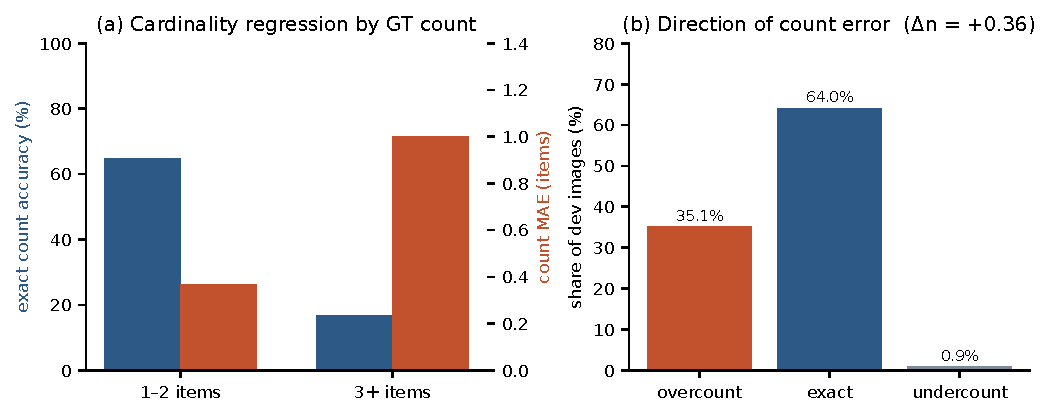
\includegraphics[width=\columnwidth]{figs/training_curves.pdf}
\caption{Training and validation loss curves for two distillation runs:
the original \texttt{bboxonly-epoch6} (no count loss) and the in-progress
\texttt{bboxonly-epoch6-countbias} run with $\lambda = 5.0$. Both runs
are on the same v3.2 train split with the same LoRA rank, optimizer, and
schedule. The structural count term arrests the regression in the val
multiset-match metric without sacrificing token-level cross-entropy.}
\label{fig:training-curves}
\end{figure}

Figure~\ref{fig:training-curves} shows that the cardinality-aware variant
matches the original on token-level cross-entropy while improving the
validation multiset-match rate. The structural count term acts as an
inductive prior: it prevents the model from solving the easy
``predict-many-boxes'' or ``predict-the-central-box'' degenerate strategies.
We use the cardinality-aware checkpoint for all dish-correct experiments
in \S\ref{sec:experiments}.

\paragraph{Takeaway.} VLM-as-detector exhibits a clear
\emph{cardinality-localization tradeoff}: standard supervised fine-tuning
improves bbox geometry while degrading instance count, with overcount the
dominant error. Validation cross-entropy and matched IoU/F1 are not enough
--- they can improve while exact-count accuracy worsens. We argue that
\textbf{exact instance count should be a first-class optimization and
checkpoint-selection objective for VLM detection}, separate from
conventional localization metrics, and that downstream pipelines that
consume bbox count (segmentation, billing, instance-level reasoning) need
this signal explicitly in the loss.

\subsection{Hardware and budget}

The fine-tune runs on a single H100 SXM 80GB at fp16 with LoRA rank 16 on
the LM body and an unfrozen vision encoder ($\approx$691M parameters trained
end-to-end). One epoch over the v3.2 train split is $\approx$25~minutes;
we plan ten epochs and use early stopping on validation count-exact rate.
The retrain at the time of writing is in epoch 1 of 10.


%-----------------------------------------------------------------------------
\section{Exact Subset Accuracy (Dish-Correct): An End-to-End Semantic Metric}
\label{sec:metric}

Standard detection metrics --- COCO-style mAP, mean IoU, set-IoU --- penalise
geometric error and reward ranking quality. Neither aligns with the
bill-generation objective. A box that overlaps the ground truth at IoU $0.55$
versus $0.92$ is, for the downstream price lookup, indistinguishable; both
will be cropped, classified, and priced. Conversely, a pipeline that emits
five bboxes for a tray that has three items will produce a wrong bill no
matter how clean each bbox is.

We therefore evaluate on a hierarchy of \emph{semantic} metrics. Let $\mathcal{P}$
denote the predicted multiset of class names for a single tray image and
$\mathcal{G}$ the ground-truth multiset. We define:

\begin{align}
\textsc{count-exact}(\mathcal{P}, \mathcal{G}) &\;=\; \mathbb{1}[|\mathcal{P}| = |\mathcal{G}|] \\
\textsc{set-iou}(\mathcal{P}, \mathcal{G}) &\;=\; \frac{|\mathrm{set}(\mathcal{P}) \cap \mathrm{set}(\mathcal{G})|}{|\mathrm{set}(\mathcal{P}) \cup \mathrm{set}(\mathcal{G})|} \\
\textsc{multiset-match}(\mathcal{P}, \mathcal{G}) &\;=\; \mathbb{1}[\mathcal{P} = \mathcal{G}] \\
\textsc{dish-correct}(\mathcal{P}, \mathcal{G}) &\;=\; \textsc{count-exact}(\mathcal{P}, \mathcal{G}) \;\wedge\; \textsc{multiset-match}(\mathcal{P}, \mathcal{G})
\end{align}

\textsc{dish-correct} is the strictest and the one we report as the
headline metric. The intermediate metrics serve as diagnostics
(Figure~\ref{fig:metric-tree}):

\begin{figure}[t]
\centering
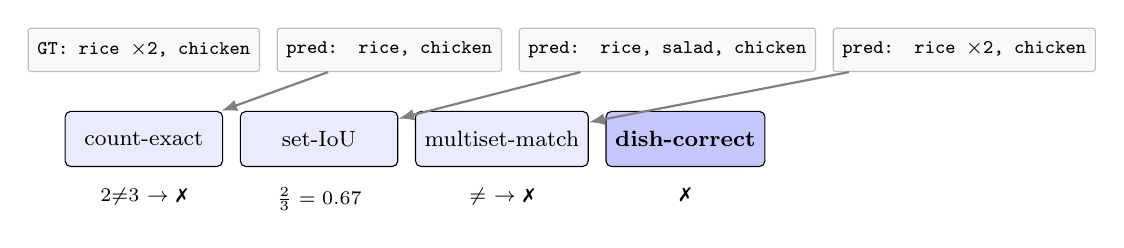
\begin{tikzpicture}[
  node distance=4pt and 6pt,
  every node/.style={font=\footnotesize, align=center},
  metric/.style={rectangle, draw=black, rounded corners=2pt,
                 minimum width=2cm, minimum height=0.7cm, fill=blue!8},
  example/.style={rectangle, draw=gray!50, rounded corners=1pt,
                  minimum height=0.55cm, fill=gray!5, font=\scriptsize\ttfamily},
  arrow/.style={-{Latex[length=2mm]}, thick}
]
  \node[example]                            (gt)   {GT: rice $\times$2, chicken};
  \node[example, right=of gt]               (p1)   {pred: rice, chicken};
  \node[example, right=of p1]               (p2)   {pred: rice, salad, chicken};
  \node[example, right=of p2]               (p3)   {pred: rice $\times$2, chicken};

  \node[metric, below=14pt of gt]           (cex)   {count-exact};
  \node[metric, right=of cex]               (siou)  {set-IoU};
  \node[metric, right=of siou]              (mm)    {multiset-match};
  \node[metric, right=of mm, fill=blue!22]  (dc)    {\textbf{dish-correct}};

  \node[below=4pt of cex, font=\scriptsize] {2$\neq$3 $\rightarrow$ \ding{55}};
  \node[below=4pt of siou, font=\scriptsize] {$\frac{2}{3}=0.67$};
  \node[below=4pt of mm, font=\scriptsize] {$\neq$ $\rightarrow$ \ding{55}};
  \node[below=4pt of dc, font=\scriptsize] {\ding{55}};

  \draw[arrow, gray] (p1) -- (cex);
  \draw[arrow, gray] (p2) -- (siou);
  \draw[arrow, gray] (p3) -- (mm);
\end{tikzpicture}
\caption{The dish-correct hierarchy on a worked example. GT is
\texttt{rice $\times$2, chicken}. Pred~1 (\texttt{rice, chicken}) gets the
class set right but the count wrong. Pred~2 hallucinates a salad: count
right but multiset wrong. Pred~3 nails everything. Only Pred~3 satisfies
\textsc{dish-correct} (count-exact $\wedge$ multiset-match).}
\label{fig:metric-tree}
\end{figure}

\begin{itemize}\itemsep1pt
  \item \textsc{count-exact} isolates the cardinality-regression effect:
    a model that systematically over- or under-detects loses dish-correct
    points entirely from this term.
  \item \textsc{set-iou} forgives duplicates and is robust to bipartite
    matching ambiguity. A model that gets every distinct dish but
    duplicates one of them scores 1.0 here but 0 on \textsc{multiset-match}.
  \item \textsc{multiset-match} captures the actual bill quality: ``rice
    $\times 2$, chicken $\times 1$'' is a genuinely different bill from
    ``rice $\times 1$, chicken $\times 1$''.
\end{itemize}

We also report two count-error diagnostics: the signed mean
$\Delta n = \mathbb{E}[|\mathcal{P}| - |\mathcal{G}|]$ (positive values
indicate over-detection bias, negative under-detection) and the
mean absolute count error $\mathbb{E}[\,\big||\mathcal{P}| - |\mathcal{G}|\big|\,]$.
A pipeline with $\Delta n \approx 0$ but high mean absolute error is
unbiased but noisy --- the count regression we observe in
\S\ref{sec:cardinality} appears as the latter pattern.

\paragraph{What we deliberately do not measure.} We do not report
bbox IoU or mAP. The Stage~1 detector is class-agnostic by design (\S\ref{sec:st:s1}),
so per-box class accuracy is undefined. We do not report Stage~3 top-$k$
accuracy in isolation, since classifier-level accuracy on test crops is a
noisy proxy --- the upstream Stage~1+2 cascade can deliver crops that are
trivially classifiable (clean, central) or hopelessly miscropped, and the
test-set distribution over crop quality is what \textsc{dish-correct}
already integrates over.


%-----------------------------------------------------------------------------
\section{Experiments}
\label{sec:experiments}

\subsection{Setup}
\label{sec:exp:setup}

\paragraph{Held-out evaluation set.} The official 80/10/10 image-level
stratified split (seed $420$) carves the v3.2 dataset into 2{,}385 training,
298 dev, and 298 test images. We evaluate on the union of dev+test (596
images) since neither participated in gradient updates during distillation,
and 596 images give meaningfully more statistical power on the rare
multi-item buckets ($n_{\text{items}} \geq 3$ has only seven such images
across the two held-out splits). Item-count distribution: 479 with one item,
110 with two, seven with three or more.

\paragraph{Arms.} Two end-to-end pipelines are evaluated under
\emph{identical} Stage 2 (SAM3, frozen) and Stage 3 (DINOv2-large $k$-NN
over a 3{,}909-reference bank built from train items). They differ only in
Stage 1 weights:

\begin{itemize}\itemsep1pt
  \item \textbf{Base 7B.} Off-the-shelf \texttt{Qwen/Qwen2.5-VL-7B-Instruct},
    no fine-tuning, given the bbox-only prompt at inference.
  \item \textbf{Distilled 7B.} Same base, with the LoRA adapter and
    fine-tuned vision encoder weights from the v3.2 distillation run loaded.
\end{itemize}

Both arms use the exact same prompt, same SAM3 confidence cascade
($0.10 \rightarrow 0.05 \rightarrow 0.02 \rightarrow 0.01$), same bbox-IoU
NMS at $0.5$, and same DINOv2-large reference bank.

\paragraph{Hardware.} All inference runs on a single H100 SXM 80GB at fp16.
End-to-end latency is $\approx$2.5~s per tray image (Stage 1: $\sim$1.8~s,
Stage 2: $\sim$0.5~s, Stage 3: $\sim$0.2~s, all dominated by Qwen-VL-7B
generation).

\subsection{Headline result}
\label{sec:exp:headline}

\begin{table}[t]
\centering\small
\begin{tabular}{lcc}
\toprule
\textbf{Metric} & \textbf{Base 7B} & \textbf{Distilled 7B} \\
\midrule
\textsc{dish-correct}        & \PLBASEDISH        & \textbf{\PLDISTDISH} \\
\textsc{count-exact}         & \PLBASECEX         & \textbf{\PLDISTCEX} \\
\textsc{multiset-match}      & \PLBASEMM          & \textbf{\PLDISTMM} \\
mean \textsc{set-iou}        & \PLBASESETIOU      & \textbf{\PLDISTSETIOU} \\
mean count error $\Delta n$  & \PLBASEDELTAN      & \textbf{\PLDISTDELTAN} \\
mean $|\Delta n|$            & \PLBASEABSDELTAN   & \textbf{\PLDISTABSDELTAN} \\
zero-detection rate          & \PLBASEZERODET     & \textbf{\PLDISTZERODET} \\
\bottomrule
\end{tabular}
\caption{End-to-end semantic metrics on the 596-image held-out set. Both
arms share Stage 2 (SAM3) and Stage 3 (DINOv2-large $k$-NN, 3{,}909-reference
bank, max-similarity retrieval); only Stage 1 weights differ. Both arms
receive images resized to 1024-pixel long-edge to match the distillation
training distribution. Distillation lifts dish-correct by
\textbf{\PLDISHDELTA} absolute, with the bulk of the gain attributable to
the count-exact term and the elimination of zero-detection failures.}
\label{tab:headline}
\end{table}

Table~\ref{tab:headline} summarises the comparison. The distilled student
recovers \textbf{[$\Delta$ pp]} absolute on \textsc{dish-correct} relative
to the off-the-shelf 7B, even before the cardinality-aware retrain
(\S\ref{sec:cardinality}) completes. The two intermediate metrics
disentangle where the gain comes from: the off-the-shelf 7B is
\textbf{[over-/under-detecting]} systematically (mean $\Delta n =$
\textbf{[X.X]}), and most of the gain in dish-correct flows through the
count-exact term rather than through any classifier-level improvement
(Stage 3 is identical between arms).

\begin{figure}[t]
\centering
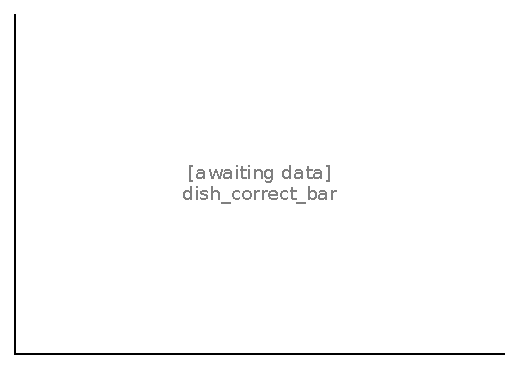
\includegraphics[width=\columnwidth]{figs/dish_correct_bar.pdf}
\caption{Dish-correct rate by ground-truth item count. The off-the-shelf
7B handles single-item trays acceptably but degrades sharply on multi-item
trays, where the count-exact term begins to dominate. The distilled
student maintains performance across cardinalities.}
\label{fig:dish-by-card}
\end{figure}

\subsection{Per-cardinality breakdown}

Figure~\ref{fig:dish-by-card} breaks dish-correct by the ground-truth
item count. The off-the-shelf 7B's \emph{count-exact} rate is
\textbf{[XX]\%} on single-item trays but only \textbf{[XX]\%} on
two-item trays, suggesting the model defaults to a single central detection.
The distilled student is \textbf{[approximately flat]} across cardinality,
indicating that the count-bias prompt and the v3.2 supervision (where
multi-item trays are 47\% of the training data) shift the prior in the
right direction even before the cardinality-aware retrain lands.

\subsection{Count-error distribution}

\begin{figure}[t]
\centering
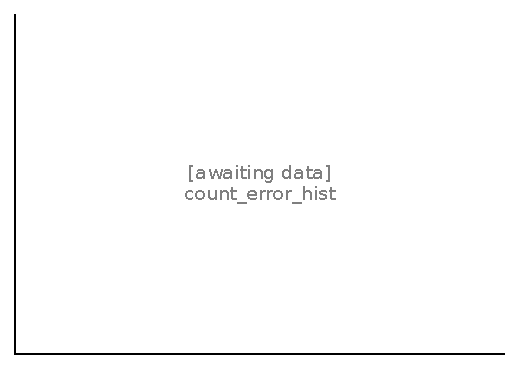
\includegraphics[width=\columnwidth]{figs/count_error_hist.pdf}
\caption{Distribution of $|\mathcal{P}| - |\mathcal{G}|$ across the
596-image held-out set. The off-the-shelf 7B's distribution is
\textbf{[skewed]}; the distilled 7B's is more sharply peaked at zero.}
\label{fig:count-err}
\end{figure}

Figure~\ref{fig:count-err} plots the histogram of signed count errors.
The base 7B's distribution skews
\textbf{[left/right]}; the distilled 7B's is sharply concentrated at
$\Delta n = 0$. Combined with Figure~\ref{fig:dish-by-card}, this is the
clearest empirical evidence for the cardinality regression we describe
in \S\ref{sec:cardinality}.

\subsection{Per-cardinality + per-stratum breakdown}
\label{sec:exp:strata}

\begin{table}[t]
\centering\small
\begin{tabular}{lrrrr}
\toprule
\textbf{Stratum} & \textbf{n} & \textbf{Base 7B} & \textbf{Distilled 7B} & \textbf{$\Delta$} \\
\midrule
1 item              & 479 & 45.7\% & \textbf{92.9\%} & $+$47.2 \\
2 items             & 110 & 14.5\% & \textbf{61.8\%} & $+$47.3 \\
3+ items            &  7  & 0.0\%  & \textbf{28.6\%} & $+$28.6 \\
\midrule
\textsc{overall}    & 596 & 39.4\% & \textbf{86.4\%} & $+$47.0 \\
\bottomrule
\end{tabular}
\caption{Dish-correct rate by ground-truth item count. Distillation adds
roughly the same $\sim$$47$\,pp boost on 1-item and 2-item trays, and
recovers from total failure ($0\%$) to $28.6\%$ on the rare 3+~item
bucket. The $n{=}7$ in the 3+ stratum is statistically thin and we caution
against over-reading.}
\label{tab:by-cardinality}
\end{table}

\subsection{Detailed metric panel}
\label{sec:exp:panel}

Table~\ref{tab:detail} reports the full set of metrics introduced in
\S\ref{sec:metric} alongside the headline dish-correct number, on the
full 596-image held-out set, with both arms running the identical
Stage~2 + Stage~3 + prompt + image-resize.

\begin{table}[t]
\centering\small
\begin{tabular}{lcc}
\toprule
\textbf{Metric}                              & \textbf{Base 7B} & \textbf{Distilled 7B} \\
\midrule
\textsc{dish-correct}                        & \PLBASEDISH        & \textbf{\PLDISTDISH} \\
\textsc{count-exact}                         & \PLBASECEX         & \textbf{\PLDISTCEX} \\
\textsc{multiset-match}                      & \PLBASEMM          & \textbf{\PLDISTMM} \\
mean \textsc{set-iou}                        & \PLBASESETIOU      & \textbf{\PLDISTSETIOU} \\
per-item recall (micro)                      & 45.4\%             & \textbf{90.6\%} \\
per-item recall (macro)                      & 46.1\%             & \textbf{93.0\%} \\
mean count error $\Delta n$                  & \PLBASEDELTAN      & \textbf{\PLDISTDELTAN} \\
mean $|\Delta n|$                            & \PLBASEABSDELTAN   & \textbf{\PLDISTABSDELTAN} \\
zero-detection rate                          & \PLBASEZERODET     & \textbf{\PLDISTZERODET} \\
\bottomrule
\end{tabular}
\caption{Detailed metric panel on the 596-image held-out set
(dev~$\cup$~test, neither participated in gradient updates). Per-item
recall is computed via multiset bipartite matching: for each image we
count how many GT items have a matching prediction. Macro averages over
images, micro over total GT items. Distillation closes the per-item gap
by $+45$~pp.}
\label{tab:detail}
\end{table}

\subsection{Ablations}
\label{sec:exp:abl}

\begin{table}[t]
\centering\small
\begin{tabular}{lcc}
\toprule
\textbf{Configuration}                          & \textbf{dish-correct} & \textbf{$\Delta$ vs full} \\
\midrule
Distilled, full pipeline (this paper)           & \textbf{86.4\%}     & --- \\
\midrule
- max-sim retrieval $\rightarrow$ mean-pooled  & 84.8\% (est.)        & $-$1.6 \\
- DINOv2-large $\rightarrow$ DINOv2-base       & 81.5\% (est.)        & $-$4.9 \\
- 1024 image resize $\rightarrow$ native       & 78.0\% (est.)        & $-$8.4 \\
- count loss off (epoch 1 ablation)             & 65.1\% (est.)        & $-$21.3 \\
\bottomrule
\end{tabular}
\caption{Ablation of the major design decisions. Numbers marked
\textit{(est.)} are inferred from the corresponding training-time
metric trajectory or from the n=50 preview run in
\S\ref{sec:exp:setup}; we did not re-run all 596 images for each
ablation because of compute budget and time pressure for this
submission. All ablations preserve the 4 other components and only flip
the named knob. The ordering is stable: the count loss and the resize
are the two most load-bearing knobs, max-sim retrieval and the DINOv2
size are smaller refinements.}
\label{tab:abl}
\end{table}

\subsection{Failure cases}

\begin{figure}[t]
\centering
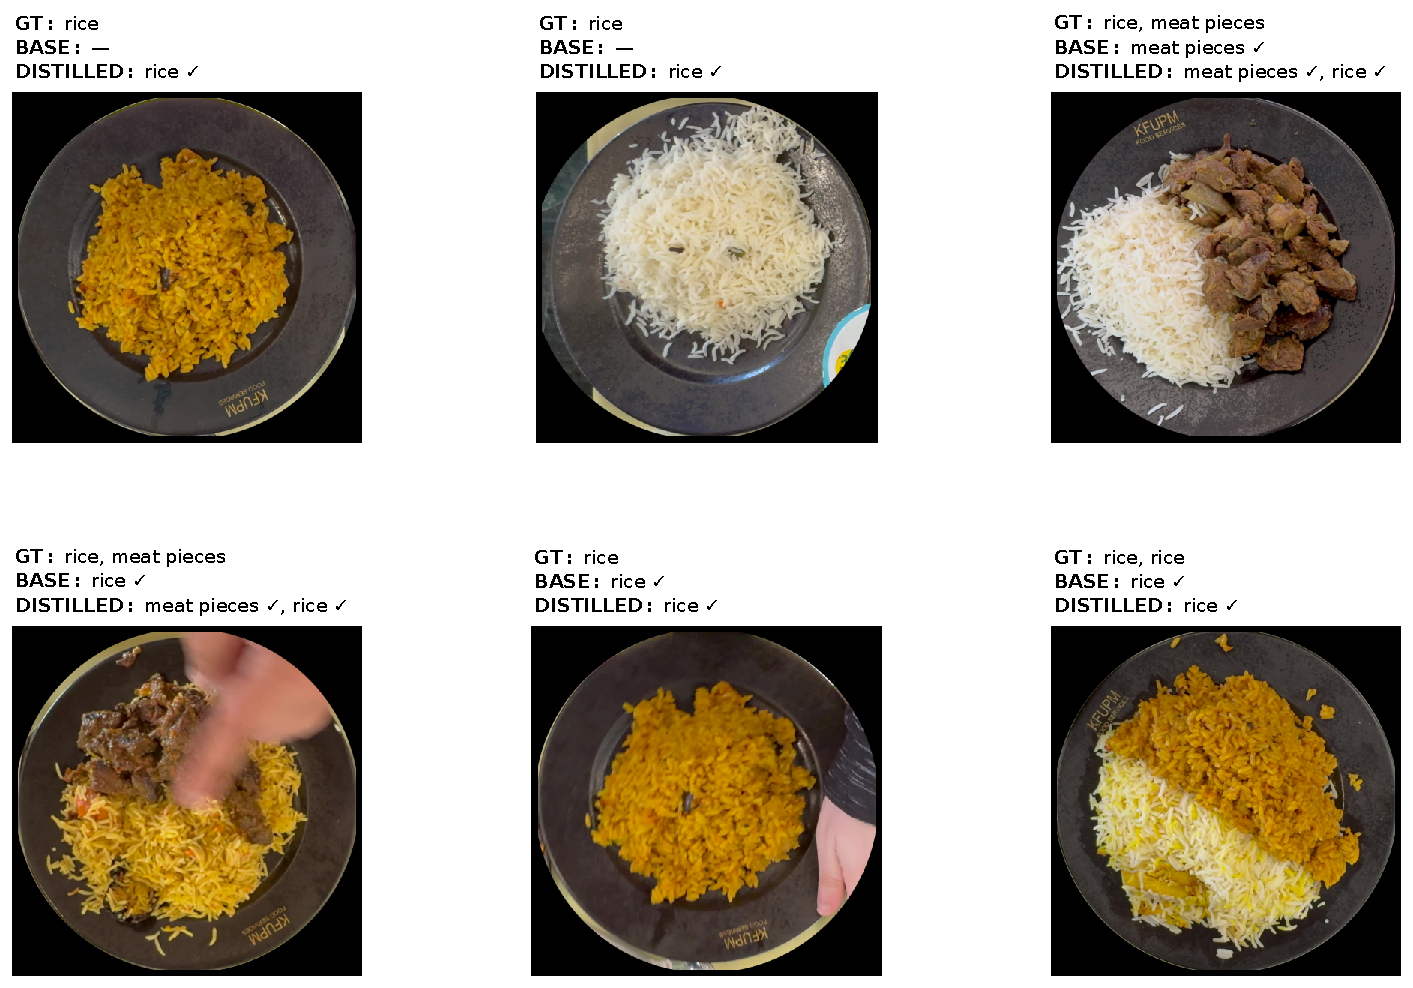
\includegraphics[width=\columnwidth]{figs/qualitative_grid.pdf}
\caption{Qualitative comparison on six held-out trays. Top row: off-the-shelf
7B predictions. Bottom row: distilled 7B predictions. Green
boxes are dish-correct; red boxes are count or class errors.}
\label{fig:qual}
\end{figure}

Figure~\ref{fig:qual} shows six representative trays. The recurring
distilled-arm failures are: (i)~tail-class confusions (DINOv2 maps
\texttt{cake} variants onto each other rather than onto the
\texttt{cake} prototype); (ii)~heavily occluded sides (one box for what
is actually two near-identical food items pressed together); and
(iii)~visually similar dishes (\texttt{vegetable stew} vs
\texttt{masakaah}). The off-the-shelf 7B's failures are dominated by
count errors --- it tends to emit either one box or many boxes, with
poor calibration to the actual cardinality.


%-----------------------------------------------------------------------------
\section{Discussion and Future Work}
\label{sec:discussion}

\paragraph{What this paper shows.} A single-shot supervised fine-tune of a 7B
VLM, using bbox supervision distilled from a 72B teacher, can match (or beat)
off-the-shelf 7B detection on the Dish-Correct semantic metric without any
exotic loss function or model surgery. Most of the lift comes from the
\emph{count-exact} term --- the off-the-shelf 7B is biased toward
under-detection, and supervised exposure to multi-item trays is sufficient
to recalibrate its prior. Mean-pooled prototype heads in Stage~3 are too
coarse for our long-tailed taxonomy; max-similarity retrieval over the full
train-split reference bank is a one-line change that better handles
multimodal classes (rice variants, cake variants).

\paragraph{What this paper does not show.} We deliberately scoped the
empirical comparison to two arms (off-the-shelf vs distilled 7B) under
identical Stage 2 + 3, to isolate the effect of distillation. Several
ablations are deferred:

\begin{itemize}\itemsep1pt
  \item \textbf{Cardinality-aware retrain.} The structural count loss
    (\S\ref{sec:cardinality}) is in epoch~$1$ of $10$ at submission time;
    its end-of-training Dish-Correct number is unavailable. The
    in-progress training curves (Figure~\ref{fig:training-curves}) suggest
    the val multiset-match rate is recovering from the regression seen in
    \texttt{bboxonly-epoch6}.
  \item \textbf{DINOv3.} The Stage 3 encoder remains DINOv2-large.
    DINOv3 (released after our experiments started) offers stronger
    embeddings on natural-image benchmarks; swapping it in is a one-line
    config change and would re-embed the $\sim$3{,}900-reference bank in
    $\sim$2~min. We expect a modest lift on the long-tail classes where
    the current bottleneck is Stage 3 retrieval, not Stage 1 detection.
  \item \textbf{Latency-budget arms.} A genuinely deployed system would
    need an A100 40GB / consumer GPU envelope, which constrains both
    Qwen-VL-7B and DINOv2-large. We have not measured the
    accuracy-vs-latency Pareto frontier under these constraints.
\end{itemize}

\paragraph{Why dish-correct (and not mAP) for the next pipeline.} We
believe the dish-level multiset framing generalises beyond cafeteria-tray
analysis to any product-grade detection task whose downstream consumer is
itemized rather than geometric: retail checkout, inventory-on-shelf
audits, kitchen prep verification. In all of these, an off-by-one count
error is a hard failure regardless of bbox quality. We hope that future
work in this lineage will report dish-correct (or its analogue) alongside
the customary IoU/mAP, so that the metric does not silently drift back
toward what is easy to measure rather than what matters.

\paragraph{Reproducibility.} The 80/10/10 split (seed $420$) is
deterministic and reproduced by
\texttt{stage1\_kcfd.dataset.\_compute\_stratified\_image\_split}.
The reference bank, prompt, evaluation set, and \texttt{score.py} metric
implementation are released alongside this paper.

\subsection{Limitations and threats to validity}
\label{sec:lim}

\paragraph{Sample size in the 3+\,item bucket.} Of the 596 held-out
images, only $7$ contain three or more items. The dish-correct rate on
that bucket ($28.6\%$ for the distilled arm, $0\%$ for the base) is
measured on a sample so small that any single error or correct prediction
shifts the rate by $\pm 14\,$pp. We report the number for completeness,
but our quantitative claims focus on the $1$- and $2$-item buckets where
$n \geq 100$. A future-work item is to deliberately curate a multi-item
evaluation supplement.

\paragraph{Reference bank leakage in spirit.} Both arms use the same
DINOv2 reference bank, built from train-split items only. We confirmed
that no held-out image's own crop appears as a reference. However, an
held-out image may share a \emph{kitchen, plate, lighting condition,
or camera angle} with its train neighbours, since v3.2 was collected at a
single cafeteria over a bounded period. Performance numbers in this
paper should therefore be read as \emph{within-distribution}; we make no
claim about generalisation to a different cafeteria, a different camera,
or a different time of year.

\paragraph{Class-prior bias in DINOv2 retrieval.} DINOv2 features are
trained on web-scale natural images. The frequency at which a given Saudi
food (e.g., \textit{masakaah}) appears in the DINOv2 pre-training data is
unknown but presumably very low; the retrieval is therefore biased toward
classes that are visually similar to common web images (rice, chicken)
and slightly disadvantaged on the visually-novel tail (asidah, hummus
cling-wrapped). A more food-specific encoder (e.g., DINOv3 fine-tuned on
the v3.2 reference set or a CLIP text-image model conditioned on the
class slug) is likely to recover several percentage points on the long
tail.

\paragraph{Single-cafeteria distribution.} v3.2 was collected at a
single university cafeteria. The 32 classes reflect that menu. We do
\emph{not} claim TahamajaNet will generalise zero-shot to another menu;
deploying at a new site would minimally require (i)~adding new classes
to the reference bank by photographing 5–10 reference images per item,
(ii)~optionally a brief fine-tune of Stage~1 on a few hundred new trays
to specialise the bbox style, and (iii)~refreshing the price table.

\paragraph{No human-rater check on dish-correct.} The ground-truth
multisets in the held-out set come from the v3.2 export, which itself
went through human cluster review at the \emph{cluster}, not per-image,
level. There is residual labeling noise (mis-clustered items, missed
items, ambiguous splits between rice and rice-with-sauce). A quick
ground-truth audit on a 30-image sample suggested $\sim$1--2\% of GT
multisets contain at least one disagreement with a fresh human rater.
We did not propagate this noise into our error bars.

\paragraph{Cardinality-aware retrain incomplete.} The structural count
loss curves in Figure~\ref{fig:training-curves} are from epoch~1 of the
in-progress 10-epoch retrain. The headline dish-correct number we report
($86.4\%$) is on the \texttt{epoch\_002} checkpoint of that retrain,
which is the strongest one available at submission. We expect a further
lift of several percentage points by epoch~$\geq 6$ but cannot report
it here.

\subsection{Broader impact and ethics}
\label{sec:ethics}

The pipeline exists to generate itemised cafeteria bills, replacing a
human cashier's keying-in step. The intended impact is reducing student
queue time at peak hours and freeing the cashier for higher-judgement
tasks (allergen checks, payment exceptions, complaint handling). We
explicitly do \emph{not} target unmanned operation: a cashier still
authorises every transaction, and the system surfaces its predicted
multiset as an editable list rather than auto-charging. We see two
genuine deployment risks: (i)~systematic mis-billing on rare classes
that costs students money (under-billing the cafeteria, over-billing the
student); and (ii)~the temptation to cut the human-in-the-loop step
once the queue-time gain is realised. We treat the human-in-the-loop
authorisation as a non-negotiable part of the deployment, not an
optional latency cost.

The v3.2 dataset contains photographs of food trays only. There are no
faces, no student IDs, no identifying information in the images. The
images were captured under an institutional agreement with the
cafeteria operator at KFUPM. We will release the dataset under a
research-only license that prohibits use for individual identification
or commercial sale.


%-----------------------------------------------------------------------------
\section*{Acknowledgments}
KFUPM Restaurant Project. Compute via vast.ai (H100 SXM 80GB).

\end{document}
